\iffalse
\let\negmedspace\undefined
\let\negthickspace\undefined
\documentclass[a4,12pt,twocolumn]{IEEEtran}
%\documentclass[conference]{IEEEtran}
%\IEEEoverridecommandlockouts
% The preceding line is only needed to identify funding in the first footnote. If that is unneeded, please comment it out.
\usepackage{cite}
\usepackage{amsmath,amssymb,amsfonts,amsthm}
\usepackage{algorithmic}
\usepackage{graphicx}
\usepackage{textcomp}
\usepackage{xcolor}
\usepackage{txfonts}
\usepackage{listings}
\usepackage{enumitem}
\usepackage{mathtools}
\usepackage{gensymb}
\usepackage[breaklinks=true]{hyperref}
\usepackage{tkz-euclide} % loads  TikZ and tkz-base
\usepackage{listings}
\usepackage{empheq}
\usepackage[utf8]{inputenc}
\usepackage{pgfplots}
\usepackage{mathrsfs}
\usepackage{multicol}
\usepackage{array}
%\usepackage{setspace}
%\usepackage{gensymb}
%\doublespacing
%\singlespacing

%\usepackage{graphicx}

\DeclareMathOperator*{\Res}{Res}
%\renewcommand{\baselinestretch}{2}
\renewcommand\thesection{\arabic{section}}
\renewcommand\thesubsection{\thesection.\arabic{subsection}}
\renewcommand\thesubsubsection{\thesubsection.\arabic{subsubsection}}

\renewcommand\thesectiondis{\arabic{section}}
\renewcommand\thesubsectiondis{\thesectiondis.\arabic{subsection}}
\renewcommand\thesubsubsectiondis{\thesubsectiondis.\arabic{subsubsection}}

% correct bad hyphenation here
\hyphenation{op-tical net-works semi-conduc-tor}
\def\inputGnumericTable{}                                 %%

\lstset{
%language=C,
frame=single, 
breaklines=true,
columns=fullflexible
}
%\lstset{
%language=tex,
%frame=single, 
%breaklines=true
%}

\begin{document}
%


\newtheorem{theorem}{Theorem}[section]
\newtheorem{problem}{Problem}
\newtheorem{proposition}{Proposition}[section]
\newtheorem{lemma}{Lemma}[section]
\newtheorem{corollary}[theorem]{Corollary}
\newtheorem{example}{Example}[section]
\newtheorem{definition}[problem]{Definition}
%\newtheorem{thm}{Theorem}[section] 
%\newtheorem{defn}[thm]{Definition}
%\newtheorem{algorithm}{Algorithm}[section]
%\newtheorem{cor}{Corollary}
\newcommand{\BEQA}{\begin{eqnarray}}
\newcommand{\EEQA}{\end{eqnarray}}
\newcommand{\define}{\stackrel{\triangle}{=}}

\bibliographystyle{IEEEtran}
%\bibliographystyle{ieeetr}


\providecommand{\mbf}{\mathbf}
\providecommand{\pr}[1]{\ensuremath{\Pr\left(#1\right)}}
\providecommand{\qfunc}[1]{\ensuremath{Q\left(#1\right)}}
\providecommand{\sbrak}[1]{\ensuremath{{}\left[#1\right]}}
\providecommand{\lsbrak}[1]{\ensuremath{{}\left[#1\right.}}
\providecommand{\rsbrak}[1]{\ensuremath{{}\left.#1\right]}}
\providecommand{\brak}[1]{\ensuremath{\left(#1\right)}}
\providecommand{\lbrak}[1]{\ensuremath{\left(#1\right.}}
\providecommand{\rbrak}[1]{\ensuremath{\left.#1\right)}}
\providecommand{\cbrak}[1]{\ensuremath{\left\{#1\right\}}}
\providecommand{\lcbrak}[1]{\ensuremath{\left\{#1\right.}}
\providecommand{\rcbrak}[1]{\ensuremath{\left.#1\right\}}}
\theoremstyle{remark}
\newtheorem{rem}{Remark}
\newcommand{\sgn}{\mathop{\mathrm{sgn}}}
%\providecommand{\abs}[1]{\left\vert#1\right\vert}
\providecommand{\res}[1]{\Res\displaylimits_{#1}} 
%\providecommand{\norm}[1]{\left\lVert#1\right\rVert}
%\providecommand{\norm}[1]{\lVert#1\rVert}
\providecommand{\mtx}[1]{\mathbf{#1}}
%\providecommand{\mean}[1]{E\left[ #1 \right]}
\providecommand{\fourier}{\overset{\mathcal{F}}{ \rightleftharpoons}}
%\providecommand{\hilbert}{\overset{\mathcal{H}}{ \rightleftharpoons}}
\providecommand{\system}{\overset{\mathcal{H}}{ \longleftrightarrow}}
	%\newcommand{\solution}[2]{\textbf{Solution:}{#1}}
\newcommand{\solution}{\noindent \textbf{Solution: }}
\newcommand{\cosec}{\,\text{cosec}\,}
\providecommand{\dec}[2]{\ensuremath{\overset{#1}{\underset{#2}{\gtrless}}}}
\newcommand{\myvec}[1]{\ensuremath{\begin{pmatrix}#1\end{pmatrix}}}
\newcommand{\mydet}[1]{\ensuremath{\begin{vmatrix}#1\end{vmatrix}}}
%\numberwithin{equation}{section}
%\numberwithin{equation}{subsection}
%\numberwithin{problem}{section}
%\numberwithin{definition}{section}
%\makeatletter
%\@addtoreset{figure}{problem}
%\makeatother

%\let\StandardTheFigure\thefigure
\let\vec\mathbf

\title{
\Huge\textbf{Gate EE 2023}\\
\Huge\textbf{EE1205} Signals and Systems\\
}
\large\author{Nimal Sreekumar\\EE23BTECH11044}

% make the title area
\maketitle


%\tableofcontents

\bigskip

\renewcommand{\thefigure}{\arabic{figure}}
\renewcommand{\thetable}{\theenumi}
%\renewcommand{\theequation}{\theenumi}


\textbf{Question Gate 2023 EE:}
For the signals x\brak{t} and y\brak{t} shown in the figure, $z\brak{t}=x\brak{t}*y\brak{t}$ is maximum at $t=T_1$. Then $T_1$ in seconds is .......... \brak{\text{Round off to the nearest integer}}\\

\begin{tikzpicture}
\begin{axis}[xmin=-3, xmax=7, ymin=-3, ymax=3, axis lines=middle, xlabel={$t$}, title={$y\brak{t}$}]
 \addplot[blue] coordinates {(-3,0) (1,0)};
  \addplot[blue] coordinates {(1,0) (1,-2)};
   \addplot[dashed] coordinates {(0,-2) (1,-2)};
  \addplot[blue, domain=1:5] {x - 3};
  \addplot[blue] coordinates {(5,2) (5,0)};
  \addplot[blue] coordinates {(5,0) (7,0)};
  \addplot[dashed] coordinates {(0,2) (5,2)};
    \end{axis}
\end{tikzpicture}

\begin{tikzpicture}
    \begin{axis}[xmin=-3, xmax=3, ymin=-3, ymax=3, axis lines=middle, xlabel={$t$} ,title={$x\brak{t}$}]
        \addplot[blue] coordinates {(-3,0) (-1,0)};
        \addplot[blue] coordinates {(-1,0) (-1,1)};
        \addplot[blue] coordinates {(-1,1) (1,1)};
        \addplot[blue] coordinates {(1,1) (1,0)};
        \addplot[blue] coordinates {(1,0) (3,0)};
    \end{axis}
\end{tikzpicture}

\hfill (GATE EE 2023)
\solution
\fi

\begin{table}[htbp]
\centering
\renewcommand\thetable{1}
\begin{tabular}{|c|m{3.5cm}|m{3cm}|}
    \hline
    \textbf{Variable} & \textbf{values} & \textbf{Description} \\
    \hline
    $x\brak{t}$ & $u\brak{t+1}-u\brak{t-1}$ & signal 1\\
    \hline
    $ y\brak{t} $ & $y\brak{t} = 
    \begin{cases}
        t-3 & ; 1\leq n \leq 5 \\
        0 & ; otherwise \\
    \end{cases}$ & signal 2\\
    \hline
    $X\brak{s}$ & $\int_{0}^{\infty}x\brak{t}e^{-st}dt$ & Laplace transform of $x\brak{t}$\\
    \hline
   $Y\brak{s}$ & $\int_{0}^{\infty}y\brak{t}e^{-st}dt$ & Laplace transform of $y\brak{t}$ \\
    \hline
    $\mathscr{L^{-1}} \{Z(s)\}$ &$f\brak{t-c}u\brak{t-c}=\mathscr{L^{-1}}\brak{e^{-cs}F\brak{s}} $& Inverse Laplace transform \\
    \hline
\end{tabular}
\caption{Input Parameters}
\label{tab:11.9.5.32}
\end{table}

Using laplace transform,
\begin{align}
z\brak{t} &=x\brak{t}*y\brak{t}\label{eq:gate_ee_Q31.1} \\
Z\brak{s} &=X\brak{s}Y\brak{s}\label{eq:gate_ee_Q31.2} \\
X\brak{s} &= \frac{1}{s} \brak{e^{s}-e^{-s}} \label{eq:gate_ee_Q31.3}\\
Y\brak{s} &= \frac{2s+1}{s^2} \brak{e^{-s}-e^{-5s}}\label{eq:gate_ee_Q31.4}\\
Z\brak{s} &= \frac{2s+1}{s^3} \brak{1-e^{-4s}-e^{-2s}+e^{-6s}}\label{eq:gate_ee_Q31.5}
\end{align}
Now taking inverse laplace transform for each terms, $\mathscr{L^{-1}} \{Z(s)\}$
\begin{align}
&= \left( 2t + \frac{t^2}{2} \right) u(t) \nonumber \\
&\quad - \left( 2(t-4) + \frac{(t-4)^2}{2} \right)u(t-4) \nonumber \\
&\quad - \left( 2(t-2) + \frac{(t-2)^2}{2} \right)u(t-2) \nonumber \\
&\quad + \left( 2(t-6) + \frac{(t-6)^2}{2} \right)u(t-6) \nonumber
\end{align}\label{eq:gate_ee_Q31.6}
From the plot it is clear that $T_1=4$.\\
\begin{figure}[h]
\centering
   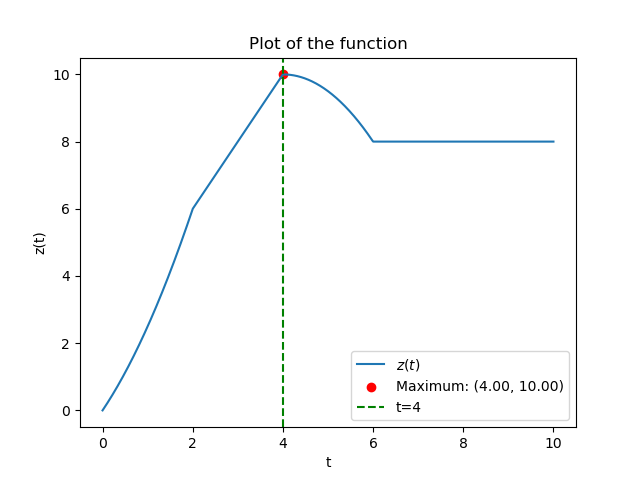
\includegraphics[width=1\linewidth]{2023/EE/31/figs/figs/gate2023EE.png}
   \caption{z\brak{t} vs. t}
   \label{fig:gate2023EE1}
 \end{figure}\\
Now in time domain,
 \begin{align}
z\brak{t} &=x\brak{t}*y\brak{t} = y\brak{t}*x\brak{t}\label{eq:gate_ee_Q31.7}\\
z\brak{t} &=\int_{-\infty}^{\infty} y\brak{\tau}x\brak{t-\tau}d\tau\label{eq:gate_ee_Q31.8}
\end{align}
$x\brak{\tau}$ is an even signal,
\begin{align}
x\brak{\tau}= x\brak{-\tau}\label{eq:gate_ee_Q31.9}\\
 x\brak{-\tau}= 
    \begin{cases}
        1 & ; -1\leq -\tau \leq 1 \\
        0 & ; \text{otherwise} \\
    \end{cases}\label{eq:gate_ee_Q31.10}
    \end{align}
    
    \begin{align}
    x\brak{-\tau} \xleftrightarrow{\text{Time shifting}} x\brak{t-\tau}\label{eq:gate_ee_Q31.11} \\
    x\brak{t-\tau}= 
    \begin{cases}
        1 & ; t-1\leq t-\tau \leq t+1 \\
        0 & ; \text{otherwise} \\
    \end{cases}\label{eq:gate_ee_Q31.12}
\end{align}\\
For $z\brak{t}$ to be maximum both $y\brak{\tau}$ and $x\brak{t-\tau}$ must be maximum,
\begin{align}
\implies t-1 &= 3 \quad \text{or} \quad t+1 = 5 \nonumber \\
t &= T_1 = 4 \nonumber
\end{align}
